% ************ Anexo  ************
%\renewcommand{\appendixname}{Anexo}
%\appendix
\chapter{Documento com as alternativas para a administração escolher }
\label{anexo:A}

Esta parte do relatório deve conter informação adicional organizada por anexos, que embora seja interessante, não faz parte do estritamente necessário ao relatório. Documentos importantes produzidos ou utilizados durante o estágio que, pela sua dimensão, não sejam colocáveis no corpo principal do relatório podem também ser incluídos em anexos.
Um exemplo possível é um capítulo com o “diário” de trabalho que o aluno teve que elaborar no moodle. Outro exemplo é um anexo com experiências mais detalhadas e complexas realizadas.

\newpage

\begin{figure}[H]
	\centering
	
\includegraphics[width=\linewidth, frame]{figuras/Alternativas/pag0.jpg}
	\caption{Capa do documento}
	\label{fig:anexo_a_capa}
\end{figure}
\newpage

\begin{figure}[H]
	\centering
	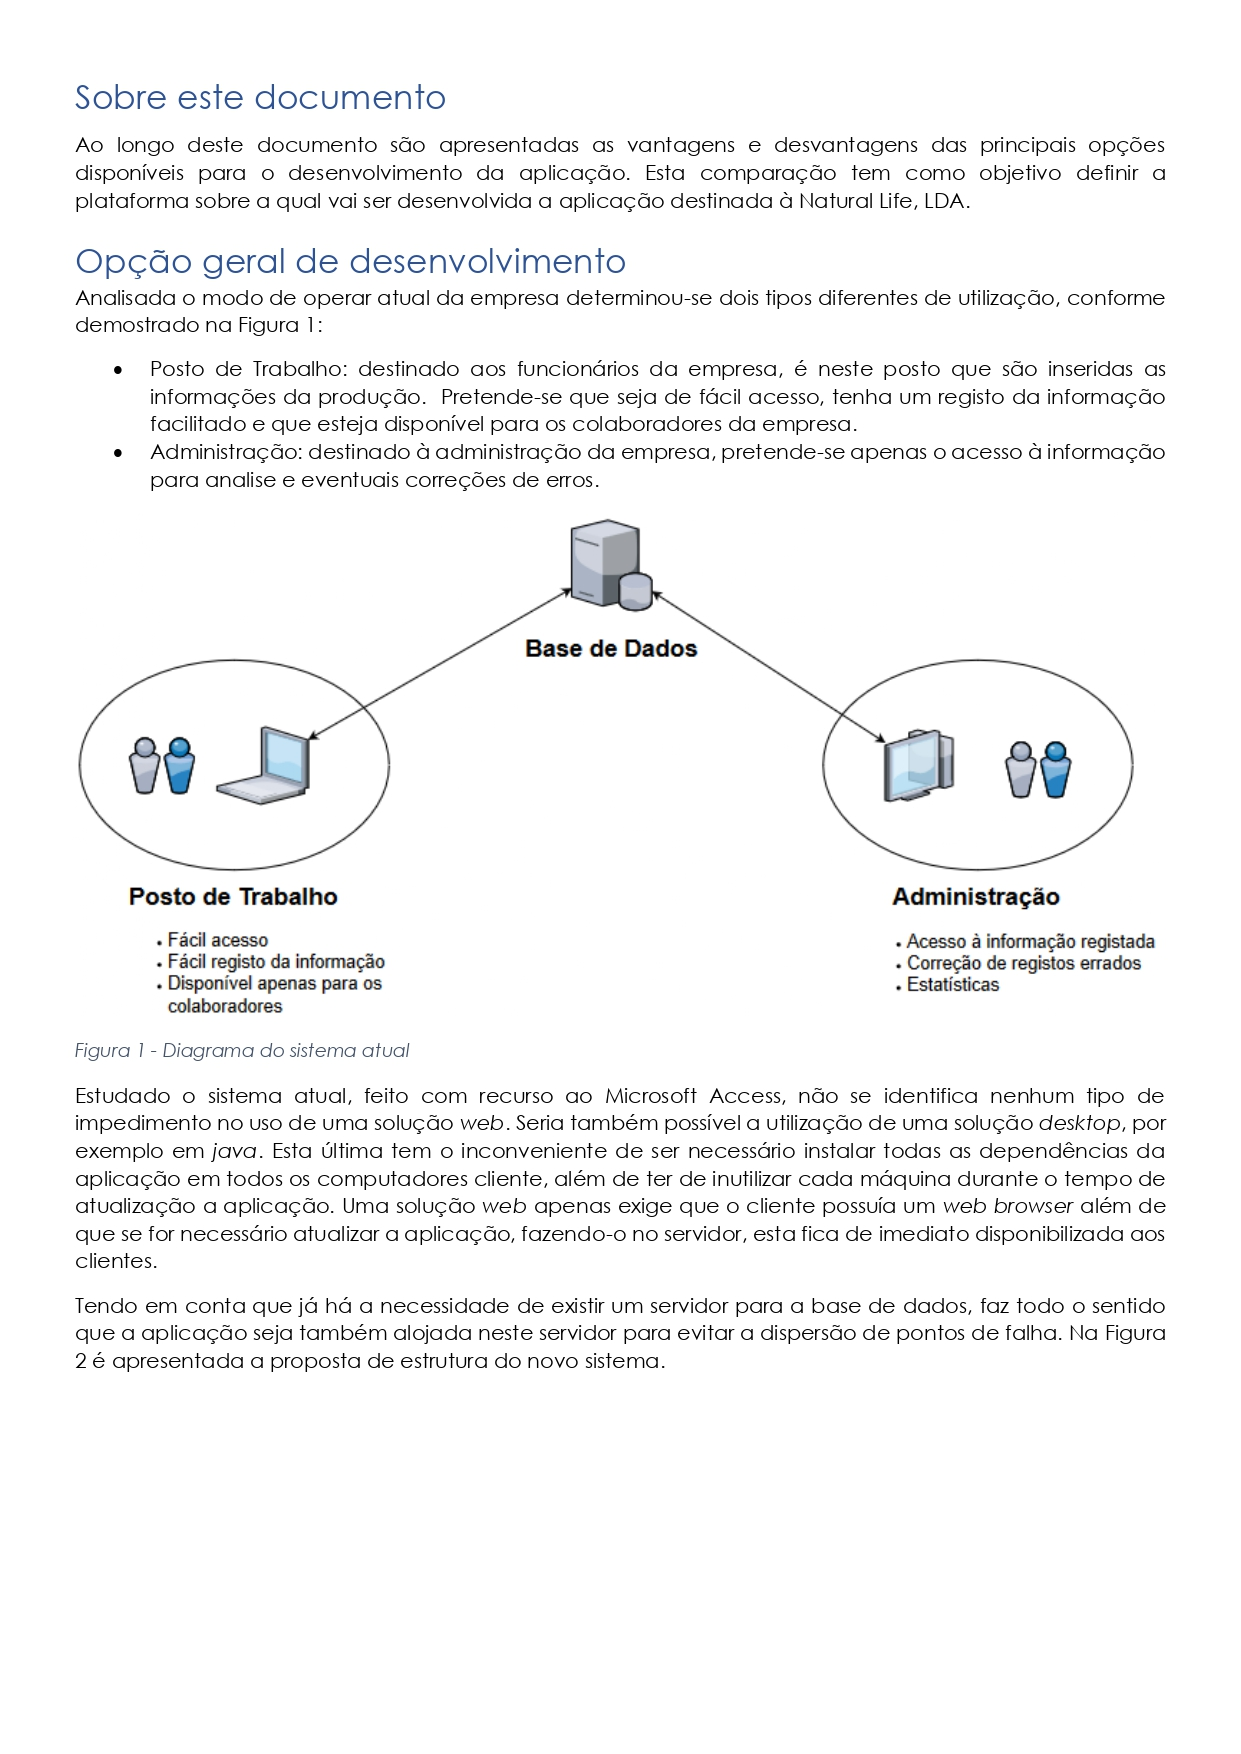
\includegraphics[width=\linewidth, frame]{figuras/Alternativas/pag1.jpg}
	\caption{Página 1}
	\label{fig:anexo_a_1}
\end{figure}
\newpage

\begin{figure}[H]
	\centering
	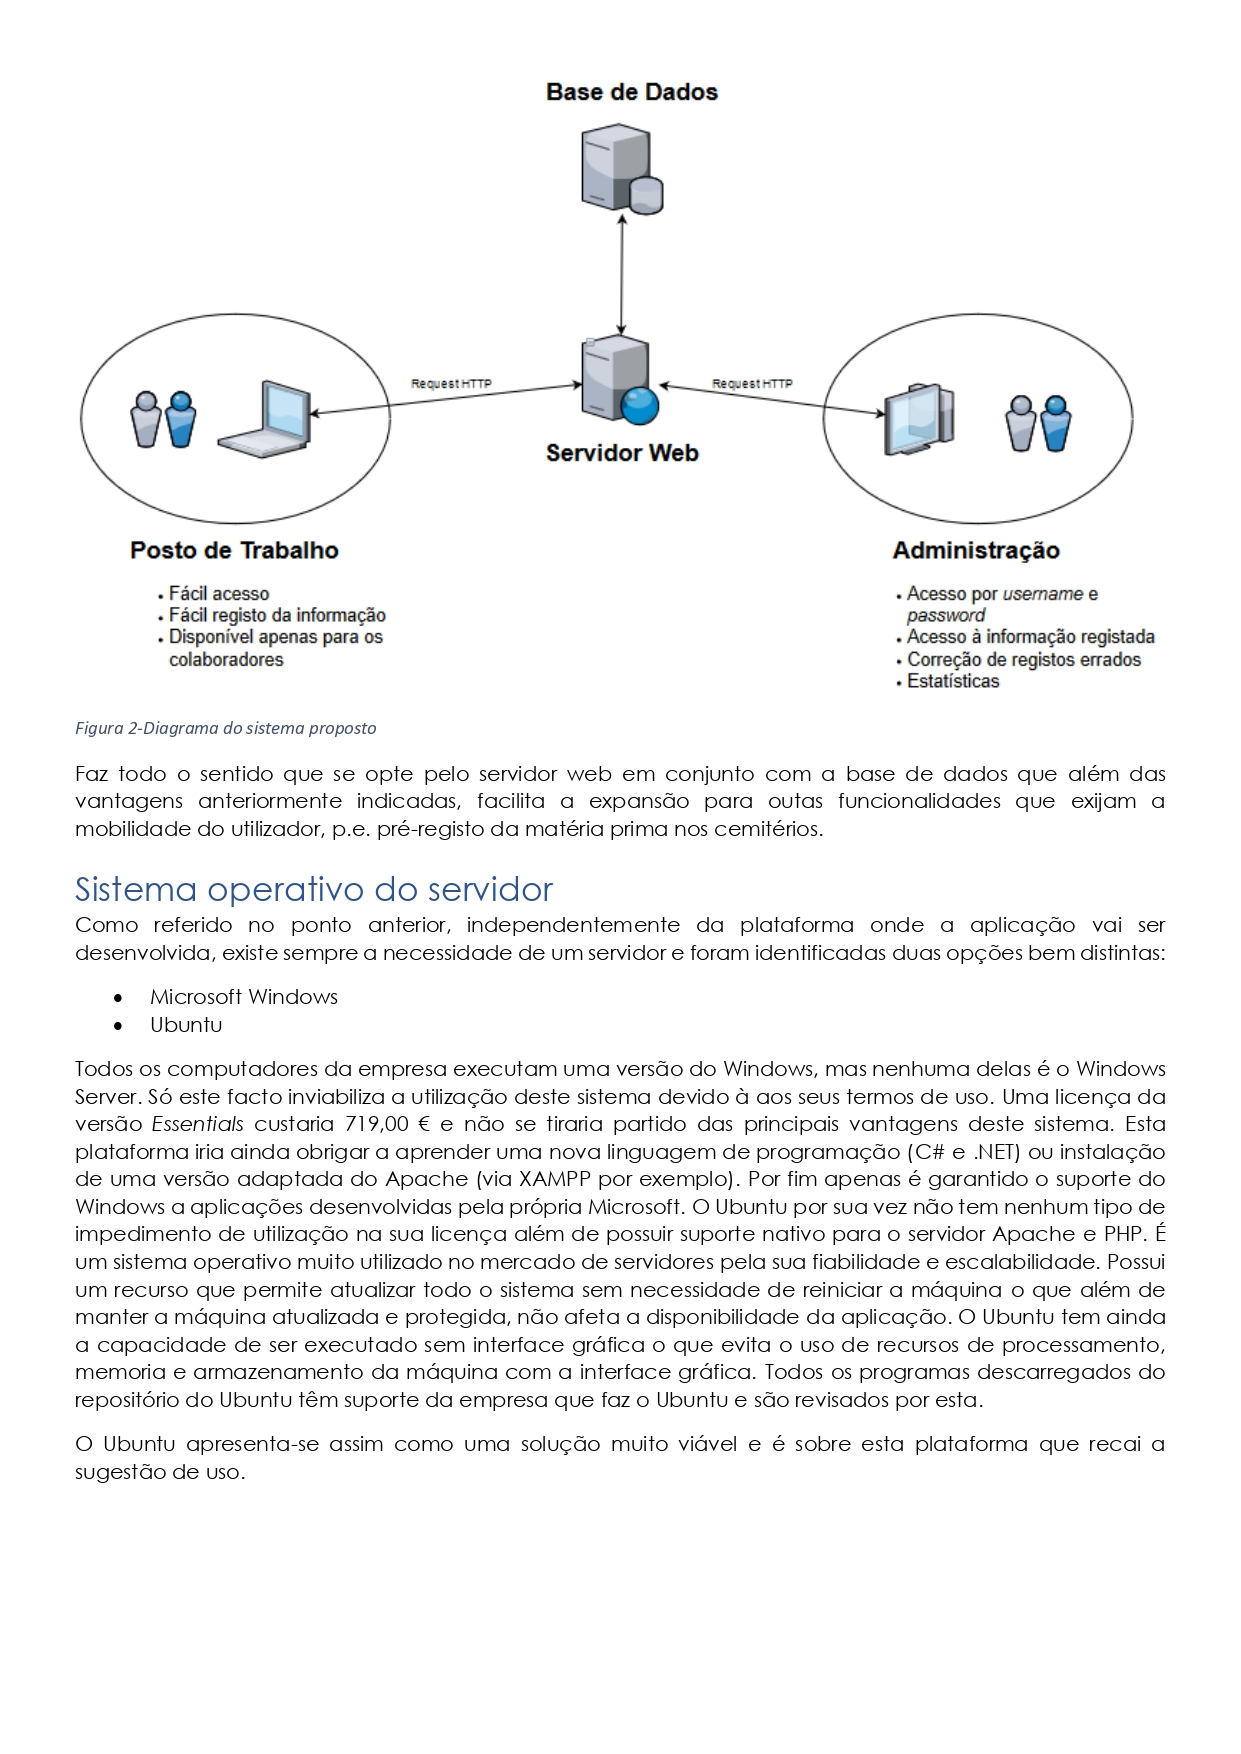
\includegraphics[width=\linewidth, frame]{figuras/Alternativas/pag2.jpg}
	\caption{Página 2}
	\label{fig:anexo_a_2}
\end{figure}
\newpage

\begin{figure}[H]
	\centering
	
\includegraphics[width=\linewidth, frame]{figuras/Alternativas/pag3.jpg}
	\caption{Página 3}
	\label{fig:anexo_a_3}
\end{figure}
\newpage

\begin{figure}[H]
	\centering
	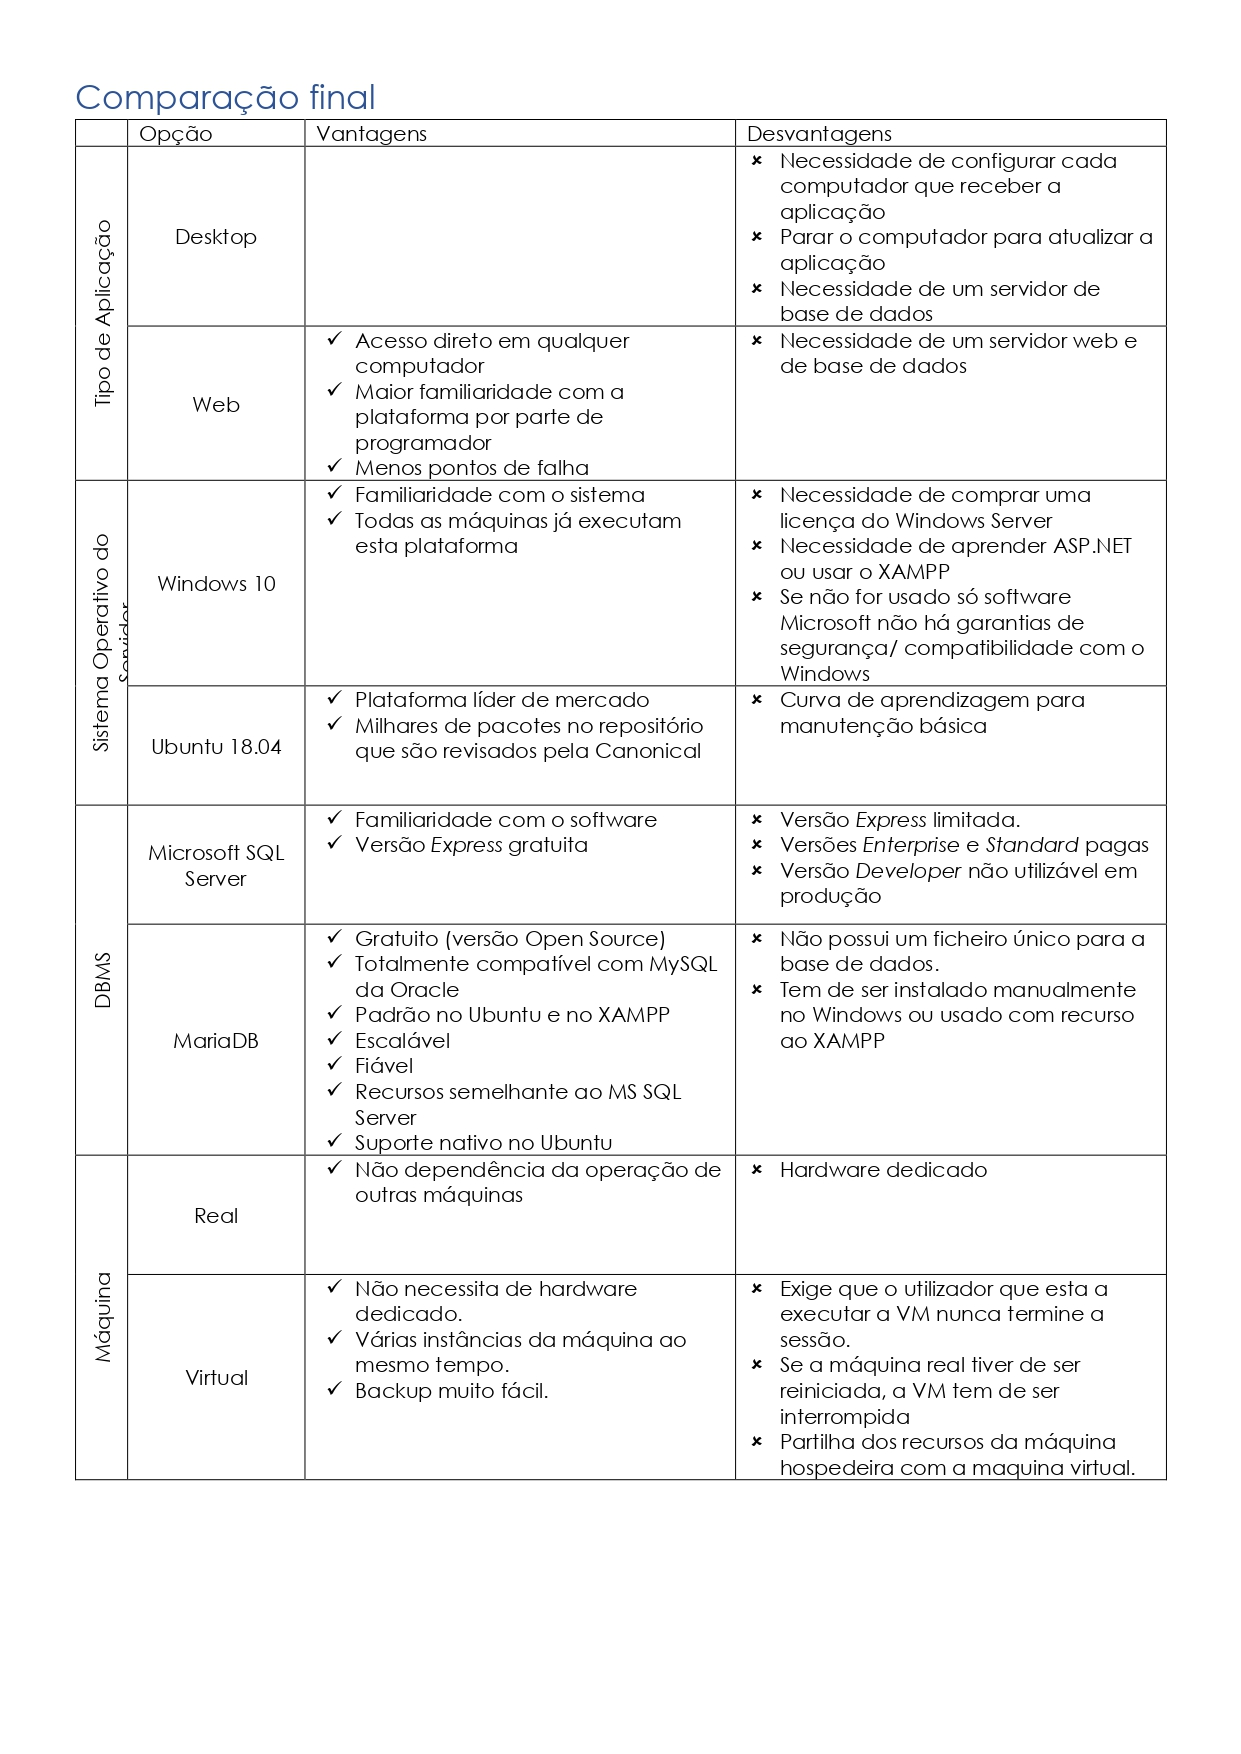
\includegraphics[width=\linewidth, frame]{figuras/Alternativas/pag4.jpg}
	\caption{Página 4}
	\label{fig:anexo_a_4}
\end{figure}
\newpage

\begin{figure}[H]
	\centering
	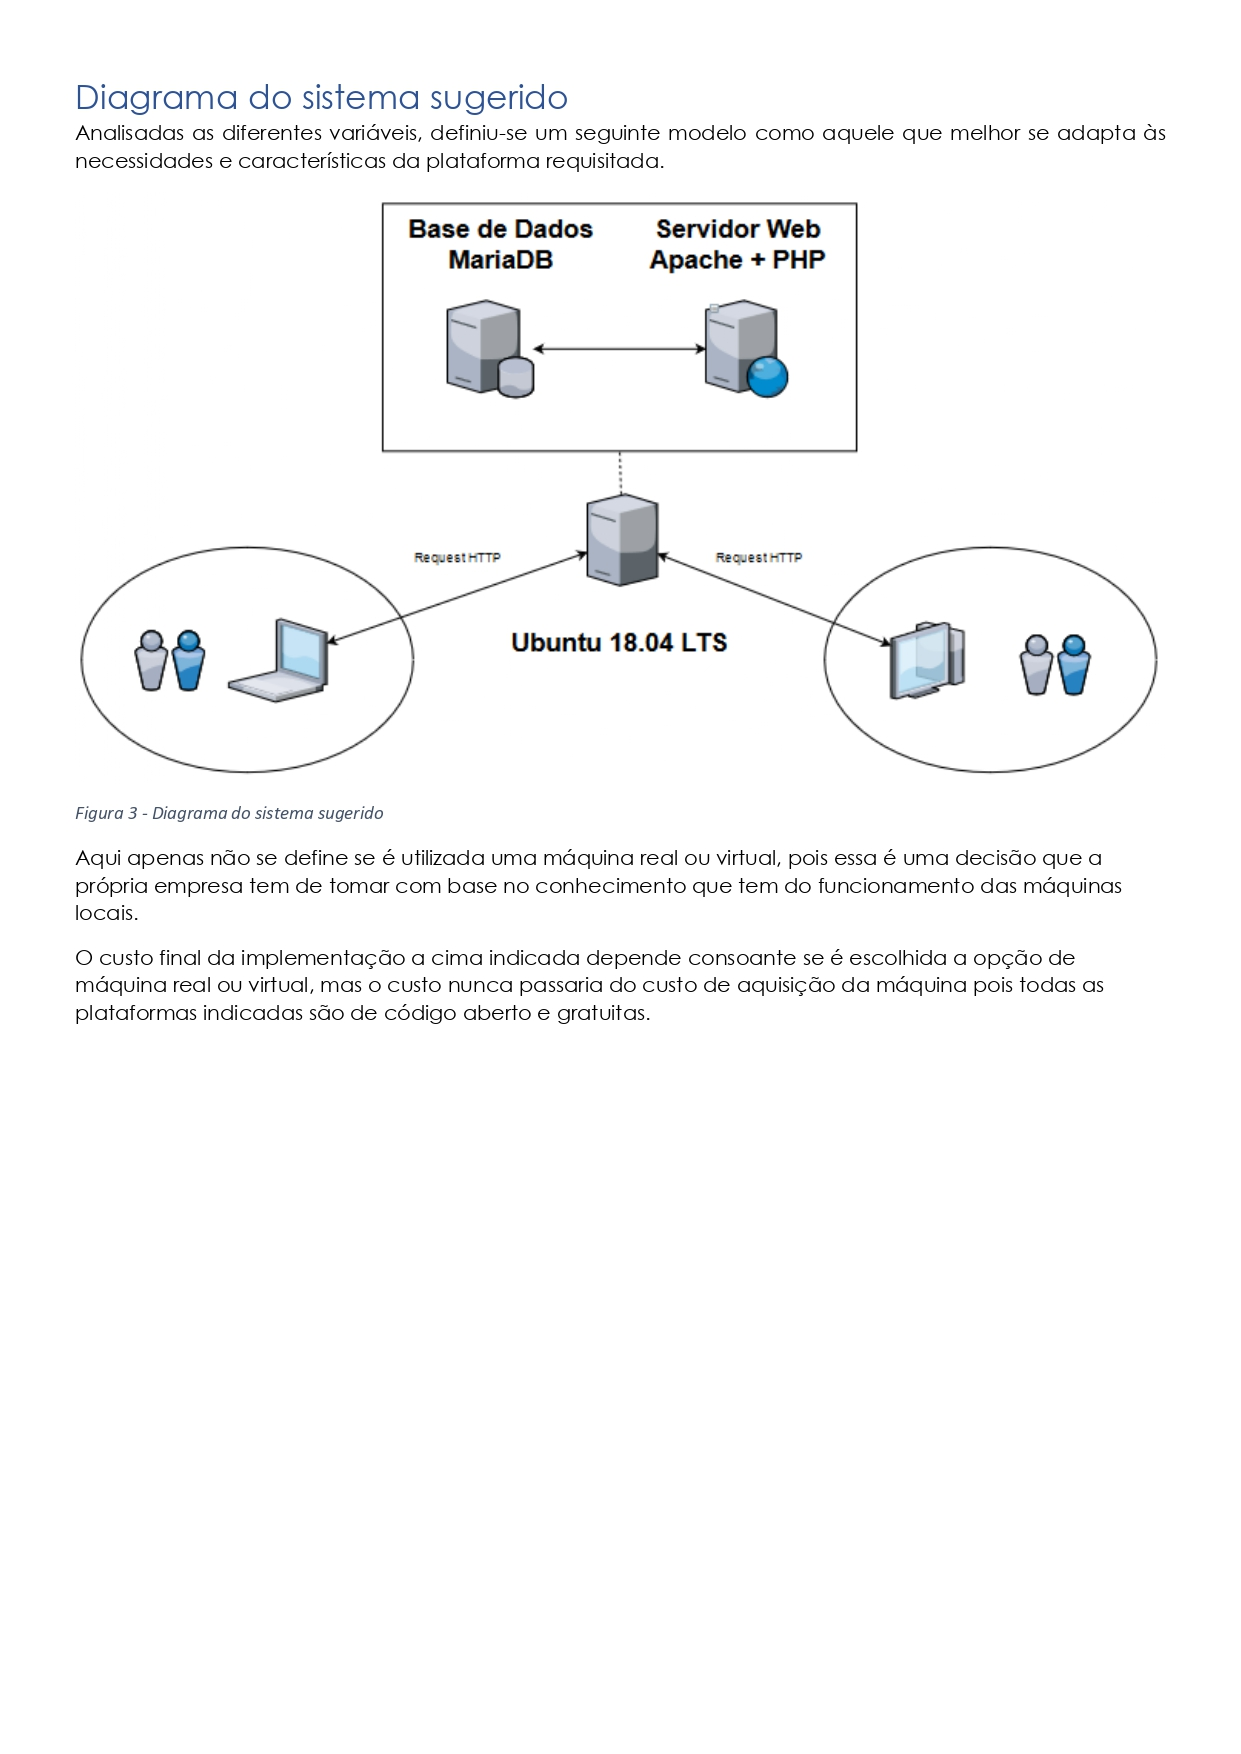
\includegraphics[width=\linewidth, frame]{figuras/Alternativas/pag5.jpg}
	\caption{Página 5}
	\label{fig:anexo_a_5}
\end{figure}
\newpage